%!TEX root=kdd15_workshop_main.tex
\section{Methodology}
While there are many possible heuristics for streaming partitioning~\cite{Stanton:2012:SGP:2339530.2339722}, the most effective by far have been \emph{weighted, greedy} approaches. We keep track of the partition assignments of vertices streamed so far ($P_i^t$ for each process $i$ at time $t$). As each vertex $v$ is streamed, we count the edges from that vertex to each partition $|P_i^t \cap N(v)|$. This intuitively maximizes \emph{modularity}, the ratio of intra-partition edges to inter-partition edges. However, using this value on its own would result in all vertices being assigned to a single, large partition. Thus, we exponentially \emph{weight} the edge counts by the size of partitions $|P_i^t|$, relatively dampening the scores for partitions that are too large (but penalizing only lightly for small differences in size). This gives us two parameters: the linear importance of partition size to the score, $\alpha$, and the exponential rate at which increasing partition size incurs a greater penalty, $\gamma$. This yields the basic `FENNEL' algorithm~\cite{tsourakakis2012fennel}:

\begin{algorithm}
 Set all $P_i$ to $\emptyset$\;
 \ForEach{$v \in V(G)$ as it arrives at time $t$}{
   $j \gets \displaystyle \argmax_{i\in\{1,\dots,p\}}|P_i^t \cap N(u)| - \alpha \frac{\gamma}{2}|P_i^t|^{\gamma-1}$\;
   Add $v$ to set $P_j^{t+1}$\;
 }
 \caption{Serial streaming FENNEL partitioner}
\end{algorithm}

Exact computation of this algorithm as described is not possible in parallel, because $P_i^{t-1}$ must be known to compute $P_i^t$. A multi-threaded approximation of this algorithm is easily performed by relaxing this requirement and using $P_i^{t-p}$ to compute $P_i^t$, where $p$ is the number of threads. This resulted in only a small drop in partition quality in our experiments.

To compute this algorithm in distributed memory, a naive approach is to constantly broadcast partition assignments as they are computed. Unless we use synchronization (which involves a massive performance hit), this results in a drastic drop in partition quality because the latency across a network is high enough that partition assignments are perpetually out of date. 

Our implementation follows the methodology of `restreaming' partitioning'~\cite{nishimura2013restream}, which shows the single-pass algorithms of FENNEL and WDG~\cite{tsourakakis2012fennel,Stanton:2012:SGP:2339530.2339722} can be repeated over the same data in the same order, yielding a convergent improvement in quality. This approach has other benefits that we utilize:

\begin{itemize}
\item Partition data is only communicated between streams, yielding high parallelism.
\item Parameters ($\alpha, \gamma)$ can be `tempered' to achieve higher-quality, balanced results that avoid immediate global minima.
\end{itemize}

\subsection{\ourmethod}
\ourmethod operates on a distributed graph $G$ in distributed CSR format. We take as input the parameters $\alpha, \gamma$, the number of partitions \numprocsparm (assumed to be equal to the number of MPI processes), the number of re-streams $\numrestreamsparm$, and the `tempering' parameter \expparm. \ourmethod then performs $\numrestreamsparm$ iterative passes over the graph (in identical random order), multiplicatively increasing the balance parameter by \expparm with each pass. This promotes a high-quality but less-balanced partition early on, while further promoting balance with subsequent pass~\cite{nishimura2013restream}. 

In between each pass, the partition information is communicated across all processors using the MPI \textsc{AllGather} primitive, which is often optimized for a given network architecture. The pseudocode for \ourmethod is shown in Algorithm~\ref{alg:grasp}.


\begin{algorithm}
\ForPar{each process $p$}{
	$vorder \gets rand\_perm(\{0,\dots,|V(G_{local})|\})$\;
	Randomly assign local vertices to partitions $P_{i,p}^0$\;
}
\For{$run \gets \{ 1 \dots \numrestreamsparm \}$} {
	\ForPar{each process $p$}{
		\ForEach{$v \in vorder$}{
			$k \gets \displaystyle \argmax_{i\in\{1,\dots,p\}}|P_{i,p}^t \cap N(u)| - \alpha \frac{\gamma}{2}|P_{i,p}^t|^{\gamma-1}$\;
			Add $v$ to set $P_{k,p}^{t+1}$\;
		}
	}
	\textsc{MPI\_AllGather} global partition assignments\;
}
 \caption{Parallel Restreaming performed by \ourmethod.}
 \label{alg:grasp}
\end{algorithm}

This method is illustrated graphically in Fig.~\ref{fig:restream}. In practice, we store the partitioning in a single compressed array, updating partition assignments in-place while storing a running count of the partition sizes. To increase accuracy we occasionally recompute global partition sizes using the \textsc{MPI\_AllReduce} primitive. 

\begin{figure}[ht]
\centering
  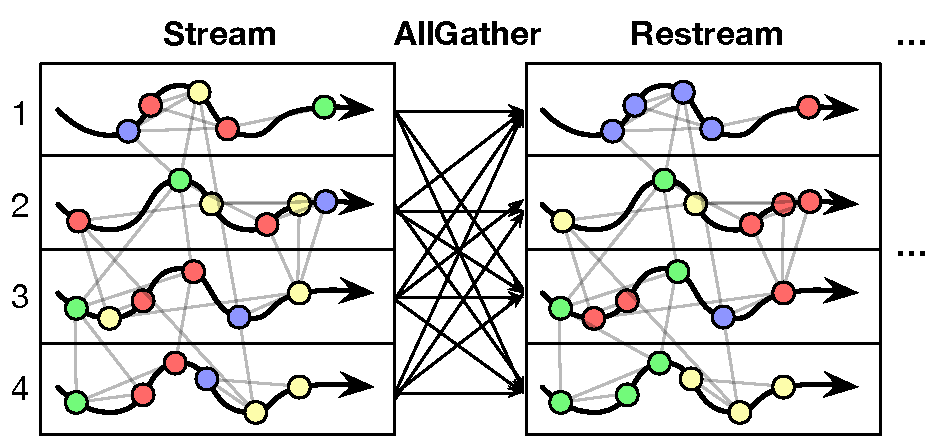
\includegraphics[width=1.0\columnwidth]{figures/restreamdiagram.pdf}
  %\caption{Partition speed of various Kronecker graphs.}
  \label{fig:restream}
  \caption{Two parallel restreaming steps on four processes.}
\end{figure}

Each process computes $O(\numrestreamsparm \cdot \frac{|E|+|V|}{p})$ work, and the network incurs a time of $\numrestreamsparm \cdot T_{allgather}(|V(G)|)$. 
